\section{Introduction}
\label{sec:introduction}
One of the most important and useful motor types in modern electronics is the BLDC (Brushless DC Motor) / PMAC (Permanent Magnet Motor). The motor achieves this status by being highly versatile, robust, low noise with a high torque. The project focuses on the controlling of a ME1117 Brush less PMAC motor for an electrical go kart. \\

The project designs the hardware shown in the green square on figure \ref{fig:Possiblesolution}. The figure show a simplified motor controller consisting of a three-phase inverter controlled by a Zynq-7000 controller.


% The solution to this problem, is of course a piece of hardware neatly designed to meet the needs of the motor. With software being able to sense and control the hardware. Such a design has been illustrated by the supervisors, and given at the start of the project as seen in figure 1. \\

\begin{figure} [H]
  \centering
  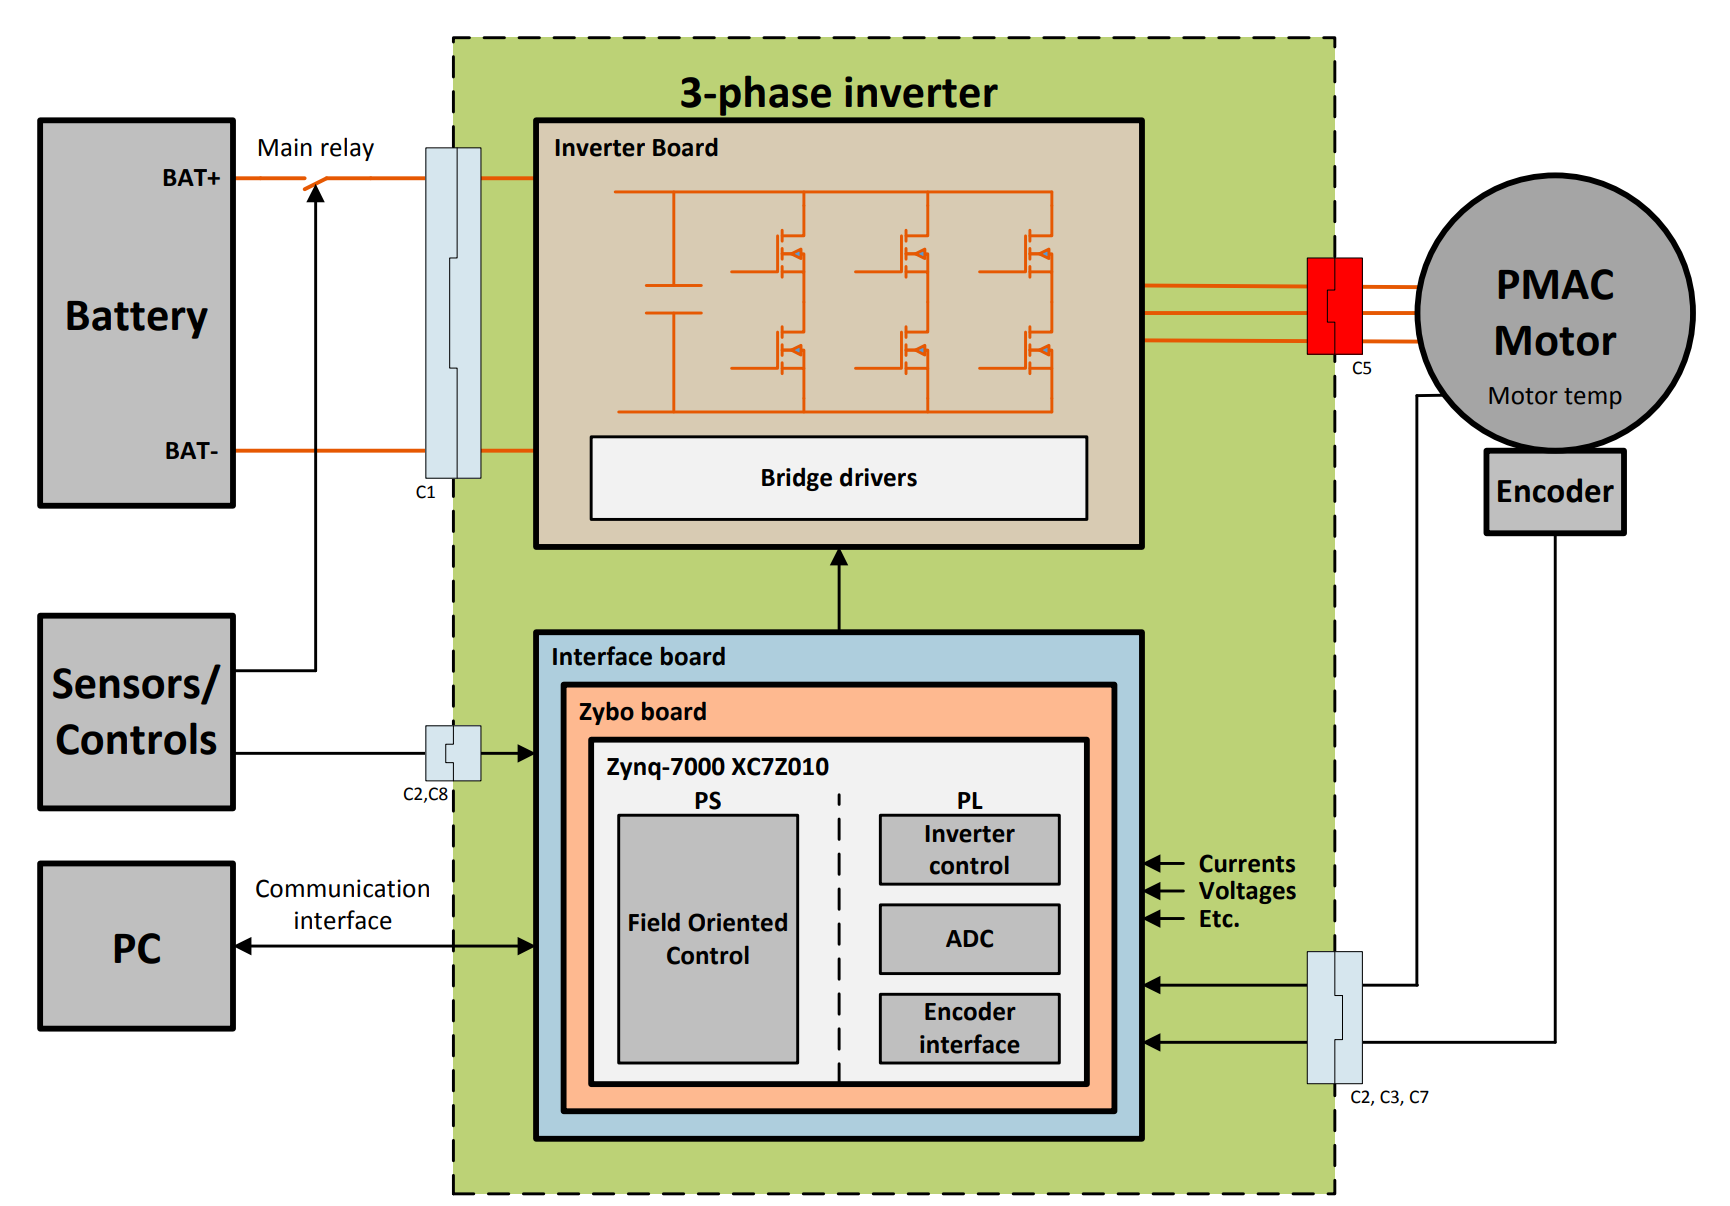
\includegraphics[width=\linewidth]{pictures/general/Project1.PNG}
  \caption{A suggestion to a possible solution given in the project description. \cite{Project 1. semester - S19}}
  \label{fig:Possiblesolution}
\end{figure}

The illustration shows how the main connections between elements could look. On the right side is the motor itself with an encoder attached to measure the rotor angle. The motor is driven by the three-phase inverter developed in this project as can be seen in the middle. Below the inverter in the green square is the Zynq controller on a Zybo training board which controls the inverter. By receiving a range of sensor signals the controller handles the control needed for the inverter to run the motor at the requested torque.

% The hardware parts is in the 3-phase inverter and a small analog board, with the software being written on a Zybo board micro-controller. The interface board is a component all ready done, it is not designed but the group, but a tool for the communication between hardware and software.

\subsection{Requirements}

\textbf{Project requirement} \\
The list below contains the requirements set for the project. Some requirements are part of the project description \cite{Project 1. semester - S19} while others are set by the group.

\begin{itemize}
\item The motor controller should only be able to control the PMAC motor in forward direction.

\item The solution must use a Zynq FPGA and a self‐designed 3‐phase inverter to control the PMAC motor.

\item There should be a control circuit, with a model of the motor and its controllers.

\item It should be possible to set and get relevant parameters through a communication interface on a computer. 

\item It is not allowed to change any mechanical or electrical parts on the kart, except replacing the Sevcon gen4 controller. 


\end{itemize}